\documentclass{ximera}[font=12pt]

\title{Subtracting Integers: Rule}   % Use xmlatex all -s to compile when SERVE refuses to work.
\author{Kelly Stady}
\license{CC: 0}         % replace with an appropriate license, or set it in xmPreamble

\begin{document}

\begin{abstract}

\end{abstract}

\maketitle
\label{xim:SubtractIntIntroActivity}

\section*{Rule for Subtracting Integers}

Our work with elevation spans demonstrated that \textbf{subtracting a number is equivalent to adding its opposite}. This rule is stated formally below.

\begin{procedure}[\textbf{Subtracting Integers}]


If $a$ and $b$ are integers, then $a-b = a + (-b).$  \\

\begin{example}

Subtracting $-12$ is equivalent to adding positive $12.$ \\
$-1 - (-12) = -1 + 12$ \\

Subtracting positive $12$ is equivalent to adding $-12.$  \\
$-1 - 12 = -1 + (-12)$

\end{example}
\end{procedure}

\begin{remark}

\begin{enumerate}

\item Once the subtraction problem has been rewritten as addition, use the rules for adding integers to find the answer.

\item When you subtract a positive number from a \emph{larger} positive number, there is no reason to rewrite the subtraction problem as
addition of the opposite.  For example, you don't need to rewrite $7-2$ as $7 + (-2)$ to figure out that the answer is $5.$  
So, \textbf{only rewrite subtraction as addition if you need to}.
\end{enumerate}

\end{remark}

\begin{problem}
Rewrite the subtraction problem as an equivalent addition problem.  Then find the answer.

\[ -6 - (-3) \]

\begin{multipleChoice}
\choice{$-6 - (-3) = 6 + 3$}
\choice{$-6 - (-3) = -6 + (-3)$}
\choice[correct]{$-6 - (-3) = -6 + 3$}
\choice{$-6 - (-3) = 6 + (-3)$}
\end{multipleChoice}


\textcolor{orange!80!black}{\textbf{Answer}}  $ = \answer{-3}$

\end{problem}


INSERT VIDEO!!!


\begin{problem}
Rewrite the subtraction problem as an equivalent addition problem.  Then find the answer.

\[ -2 - 10 \]

\begin{multipleChoice}
\choice{$-2 - 10 = 2 + (-10)$}
\choice{$-2 - 10 = 2 + 10$}
\choice[correct]{$-2 - 10 = -2 + (-10)$}
\choice{$-2 - 10 = -2 + 10$}
\end{multipleChoice}

\textcolor{orange!80!black}{\textbf{Answer}} $ = \answer{-12}$

\end{problem}

\begin{problem} 
Rewrite the subtraction problem as an equivalent addition problem. Then find the answer. 
\[ 5 - 8 \] 
\begin{multipleChoice} 
\choice{$5 - 8 = -5 + 8$}
\choice[correct]{$5 - 8 = 5 + (-8)$}  
\choice{$5 - 8 = -5 + (-8)$} 
\choice{$5 - 8 = 5 + 8$} 

\end{multipleChoice} 
\textcolor{orange!80!black}{\textbf{Answer}} $ = \answer{-3}$ 
\end{problem}

\begin{problem} 
Rewrite the subtraction problem as an equivalent addition problem. Then find the answer. 
\[ -16 - (-1) \] 
\begin{multipleChoice} 
\choice[correct]{$-16 - (-1) = -16 + 1$} 
\choice{$-16 - (-1) = -16 + (-1)$} 
\choice{$-16 - (-1) = 16 + 1$} 
\choice{$-16 - (-1) = 16 + (-1)$} 
\end{multipleChoice} 
\textcolor{orange!80!black}{\textbf{Answer}} $ = \answer{-15}$ 
\end{problem}

\begin{problem} 
Rewrite the subtraction problem as an equivalent addition problem. Then find the answer. 
\[ 30 - (-10) \] 
\begin{multipleChoice} 
\choice{$30 - (-10) = 30 + (-10)$} 
\choice[correct]{$30 - (-10) = 30 + 10$}
\choice{$30 - (-10) = -30 + 10$} 
\choice{$30 - (-10) = -30 + (-10)$} 
\end{multipleChoice} 
\textcolor{orange!80!black}{\textbf{Answer}} $ = \answer{40}$ 
\end{problem}



Write a subtraction expression to find the vertical distance between the researcher and the submarine, rewrite it as an equivalent addition problem, and find the distance.
\[ 250 - (-180) \] 
\begin{multipleChoice} 
\choice{$250 - (-180) = 250 + (-180)$} 
\choice{$250 - (-180) = -250 + 180$} 
\choice{$250 - (-180) = -250 + (-180)$} 
\choice[correct]{$250 - (-180) = 250 + 180$} 
\end{multipleChoice} 
\textcolor{orange!80!black}{\textbf{Answer}} $ = \answer{430}\text{ feet}$ 


\end{problem}

\begin{center}
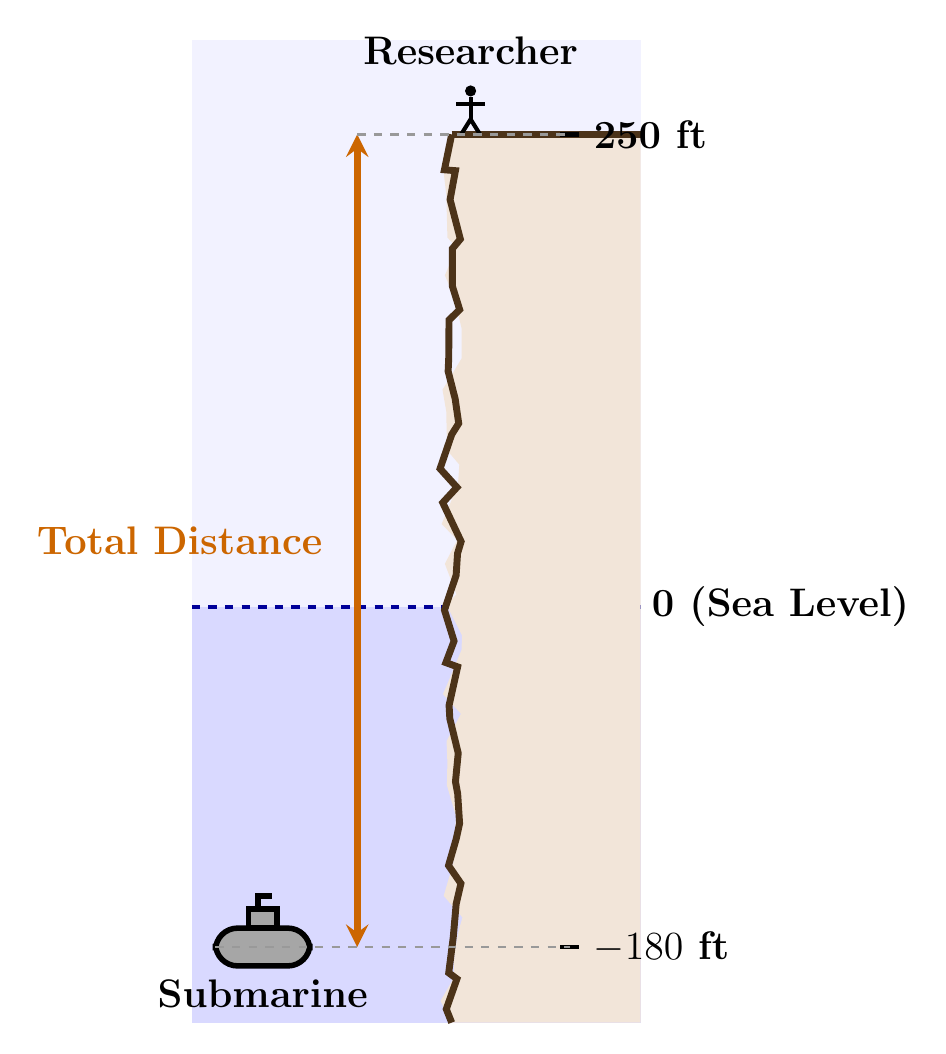
\begin{tikzpicture}[scale = 0.6, y=0.4mm, x=1mm, >=stealth, decoration={random steps, segment length=3mm, amplitude=1.5mm}]

% --- BACKGROUND & WATER ---
% Sky Block
\fill[blue!5] (-55,0) rectangle (40,300);
% Ocean Block
\fill[blue!15] (-55,-220) rectangle (40,0);
% Sea Level Line
\draw[blue!60!black, dashed, line width=1.5pt] (-55,0) -- (40,0) node[right, black] {\Large\textnormal{\textbf{0 (Sea Level)}}};

% --- SUBMARINE (Far Left) ---
% Submarine Hull
\filldraw[gray!70, draw=black, line width=2pt, rounded corners=8pt] (-50,-190) rectangle (-30,-170);
% Conning Tower
\filldraw[gray!70, draw=black, line width=2pt] (-43,-170) rectangle (-37,-160);
% Periscope
\draw[line width=2pt, black] (-41,-160) -- (-41,-153) -- (-38,-153);
% Submarine Label
\node[below, black] at (-40,-192) {\Large\textbf{Submarine}};

% --- BETTER JAGGED CLIFF (Center-Right) ---
% Ground fill with a randomized rocky edge on the left
\fill[brown!20] decorate { (0,250) -- (0,-220) } -- (40,-220) -- (40,250) -- cycle;
% Dark accent rock border line
\draw[line width=2.5pt, brown!40!black] decorate { (0,250) -- (0,-220) };
% Top cliff edge line
\draw[line width=2.5pt, brown!40!black] (0,250) -- (40,250);

% --- STICK FIGURE MAN (Top Left Edge of Cliff) ---
% Legs
\draw[line width=1.5pt, black] (2,250) -- (4,258) -- (6,250);
% Torso
\draw[line width=1.5pt, black] (4,258) -- (4,270);
% Arms
\draw[line width=1.5pt, black] (1,266) -- (7,266);
% Head
\filldraw[black] (4,273) circle (3pt);
\node[above, black, yshift=6pt] at (4,273) {\Large\textbf{Researcher}};

% --- TOTAL DISTANCE ARROW (Between Sub and Cliff) ---
\draw[<->, orange!80!black, line width=2.5pt] (-20,-180) -- (-20,250) node[midway, left=8pt, align=center] {\textnormal{\Large \textbf{Total Distance}}};

% --- ALIGNED LABELS & MARKERS (Right Side of Cliff) ---
% 250 ft Marker
\draw[ultra thick] (23,250) -- (27,250);
\node[right] at (28,250) {\Large\textnormal{\textbf{250 ft}}};

% -180 ft Marker (Perfect vertical alignment with the 250 ft text)
\draw[ultra thick] (23,-180) -- (27,-180);
\node[right] at (28,-180) {\Large\textnormal{\textbf{$-180$ ft}}};

% --- DASHED GUIDES ---
\draw[dashed, gray!80, thick] (-20,250) -- (25,250);
\draw[dashed, gray!80, thick] (-50,-180) -- (25,-180);

\end{tikzpicture}
\end{center}


\begin{problem}
How many degrees warmer is $100^\circ$F than $-80^\circ$F?  

\begin{center}
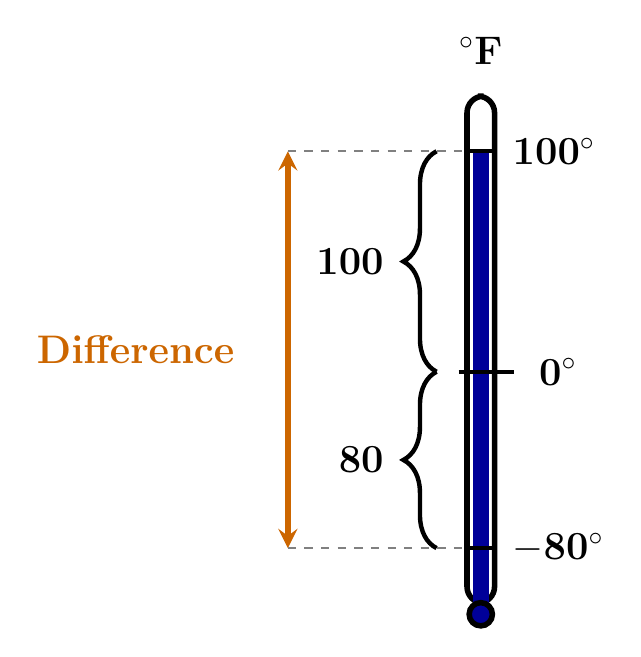
\begin{tikzpicture}[scale = 0.7, y=0.4mm, x=1mm, >=stealth]
    % --- THERMOMETER BODY ---
    % Outer Tube
    \draw[line width=2pt, black, fill=white, rounded corners=6pt] (-2.5,-105) rectangle (2.5,125);

    % Inner Blue Liquid (up to 100) for Accessibility
    \fill[blue!60!black] (-1.5,-105) -- (-1.5,100) -- (1.5,100) -- (1.5,-105) -- cycle;

    % Bulb at the bottom
    \filldraw[blue!60!black, draw=black, line width=2pt] (0,-110) circle (6pt);

    % --- VERTICAL AXIS (Labels and Units) ---
    \node[above=8pt] at (0,125) {\Large\textnormal{$^\circ$\textbf{F}}};

    % --- ZERO POINT  ---
    \draw[black, ultra thick] (-4,0) -- (6,0)
        node[right, xshift=5pt] {\Large\textnormal{\textbf{0$^\circ$}}};

    % --- KEY POINTS ---
    % 100 Degrees
    \draw[ultra thick] (-3,100) -- (3,100);
    \node[right, xshift=8pt] at (0,100) {\Large\textnormal{\textbf{100}$^\circ$}};

    % -80 Degrees
    \draw[ultra thick] (-3,-80) -- (3,-80);
    \node[right, xshift=8pt] at (0,-80) {\Large\textbf{\textnormal{$-$\textbf{80}$^\circ$}}};

    % --- BRACES ---
    \draw [decorate, decoration={brace, amplitude=12pt, raise=10pt}, ultra thick] (-3,-80) -- (-3,0)
        node [midway, left=25pt] {\Large\textnormal{\textbf{80}}};

    \draw [decorate, decoration={brace, amplitude=12pt, raise=10pt}, ultra thick] (-3,0) -- (-3,100)
        node [midway, left=25pt] {\Large \textnormal{\textbf{100}}};

    % --- TOTAL DISTANCE ARROW ---
    \draw[<->, orange!80!black, line width=2pt] (-35,-80) -- (-35,100)
        node[midway, left=15pt, align=center] {\textnormal{\Large \textbf{Difference}}};

    % --- DASHED GUIDES ---
    \draw[dashed, gray, thick] (-35,100) -- (-3,100);
    \draw[dashed, gray, thick] (-35,-80) -- (-3,-80);
\end{tikzpicture}

\xmalt{A vertical thermometer diagram labeled in degrees Fahrenheit, illustrating the distance between 
negative 80 degrees and positive 100 degrees.  The blue liquid inside the thermometer reaches up to the 
100-degree mark.  A solid black line marks the 0-degree point in the middle.  On the left side, visual 
brackets measure the distances from negative 80 to 0 (labeled 80) and from 0 to 100 (labeled 100).  
Further to the left, a double-headed orange arrow spans the entire height from negative 80 to 100, 
labeled ``Difference`` with dashed gray guide lines connecting it to the temperature marks.}
\end{center}

Write the subtraction problem.   

\begin{multipleChoice}
\choice{$100 - 80$}
\choice[correct]{$100 - (-80)$}
\choice{$-100 - 80$}
\choice{$-100 - (-80)$}
\end{multipleChoice}

Use the figure to rewrite the subtraction problem as an equivalent addition problem.  Then find the answer. 

\begin{multipleChoice}
\choice{$100 + (-80)$}
\choice{$-100 + 80 $}
\choice{$-100 + (-80)$}
\choice[correct]{$100 + 80$}
\end{multipleChoice}

\textcolor{orange!80!black}{\textbf{Answer}} $= \begin{prompt} \answer{180} \end{prompt}$ degrees

\end{problem}

\subsection*{Subtracting a Negative Number}

You may have noticed that \textbf{subtracting a negative} number is equivalent to \textbf{adding a positive} number.  
This becomes intuitive when we think in terms of money.  Imagine your checking account balance is \$900 and the 
bank realizes that they accidently charged you a \$30 $(-30)$ overdraft fee last month.  Once the bank removes 
(subtracts) the overdraft fee, your net balance increases.
\begin{eqnarray*}
900-(-30) &=& 900 + 30 \\
          &=& 930
\end{eqnarray*}
Therefore, removing a debt is the same as gaining a profit.

\end{document}